\documentclass[11pt]{article}
\usepackage[a4paper,margin=2cm]{geometry}
\usepackage{graphicx,booktabs,amsmath,float,caption}
\usepackage[hidelinks]{hyperref}
\setlength{\parskip}{4pt}\setlength{\parindent}{0pt}

\title{\textbf{PRML Lab 7 --- Neural Networks}}
\author{Aryan Tiwari (B20AI056)\\CSL2050 Pattern Recognition \& Machine Learning, Winter 2022}
\date{}

\begin{document}
\maketitle

\section*{Question 1 --- Abalone age with a two-branch PyTorch network}

\textbf{Framing.} Age is the number of rings (1--29). Many ring counts have only a few samples, so the rings are grouped into three
almost balanced age classes: \emph{young} ($\le$8 rings, 1405 samples), \emph{adult} (9--10, 1323) and \emph{old} ($\ge$11, 1447).
Two rows with \texttt{Height}~$=0$ (physically impossible) were dropped. The nominal \texttt{Sex} column (M/F/I) was one-hot encoded, giving 10
inputs, and all features were standardised using training statistics. Stratified 70/15/15 split (2921 / 627 / 627).

\textbf{Architecture.} The specification diagram was not in the question PDF I had, so I followed its text: tanh hidden layers, a sigmoid
output, and ``+'' adding the outputs of two branches. Both branches read the input. Branch A is
Linear(10$\to h$)--tanh--Linear($h\to h$)--tanh and branch B is Linear(10$\to h$)--tanh. Their sum goes through Linear($h\to3$)--sigmoid.
Each sigmoid output is an independent score for ``is it this class?'', so the loss is binary cross-entropy against one-hot targets, and the prediction
is the highest-scoring unit. Training used Adam (lr $10^{-2}$, full batch, 300 epochs), keeping the weights from the epoch with the lowest validation loss.

\textbf{Hidden size.} Validation accuracy for $h=4,8,16,32,64$ was 0.654, 0.679, \textbf{0.681}, 0.670, 0.668, so $h=16$ was chosen (675
parameters). Larger networks overfit slightly; the task is limited by noisy labels, not by model capacity.

\textbf{Result.} Test accuracy \textbf{67.9\%} (young 73.5\%, adult 53.3\%, old 76.0\%).
\begin{figure}[H]\centering
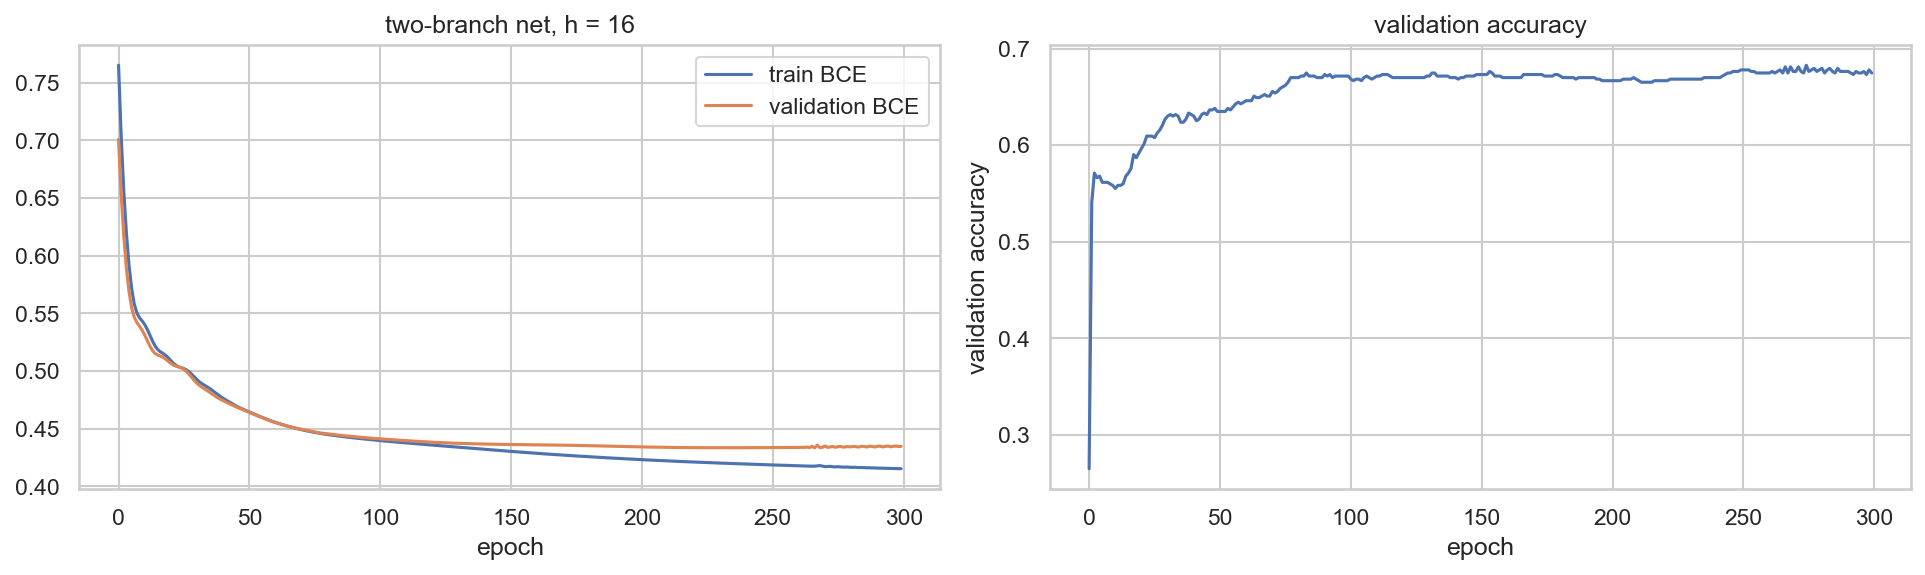
\includegraphics[width=0.85\linewidth]{figures/q1_training.png}
\caption{Training/validation loss and validation accuracy.}
\end{figure}
Most errors involve the middle class: adults are confused with both neighbours (58 predicted old, 35 young), while young and old
are rarely confused with each other (9 and 12 cases). That fits the problem: shell size and weight increase gradually with age, so the
class boundaries at 8/9 and 10/11 rings run through dense regions of feature space. Ring counts are also noisy labels, so 9 versus 10 rings is hard to
tell apart from measurements alone.

\section*{Question 2 --- Dry Bean classification with an MLP written from scratch}

\textbf{a. Data.} 13{,}611 beans, 7 varieties. The question lists ``area, perimeter, axes lengths, eccentricity, roundness, aspect ratio and convex area''.
``Axes lengths'' is two columns (major and minor), so 8 features are used. 68 exact duplicates were removed.
The classes are imbalanced (Dermason 26\%, Bombay 4\%), so the 70/15/15 split (9479 / 2032 / 2032) is \textbf{stratified}, and the class
proportions in train and test agree to 0.1\%. The features were standardised with training statistics.

\begin{figure}[H]\centering
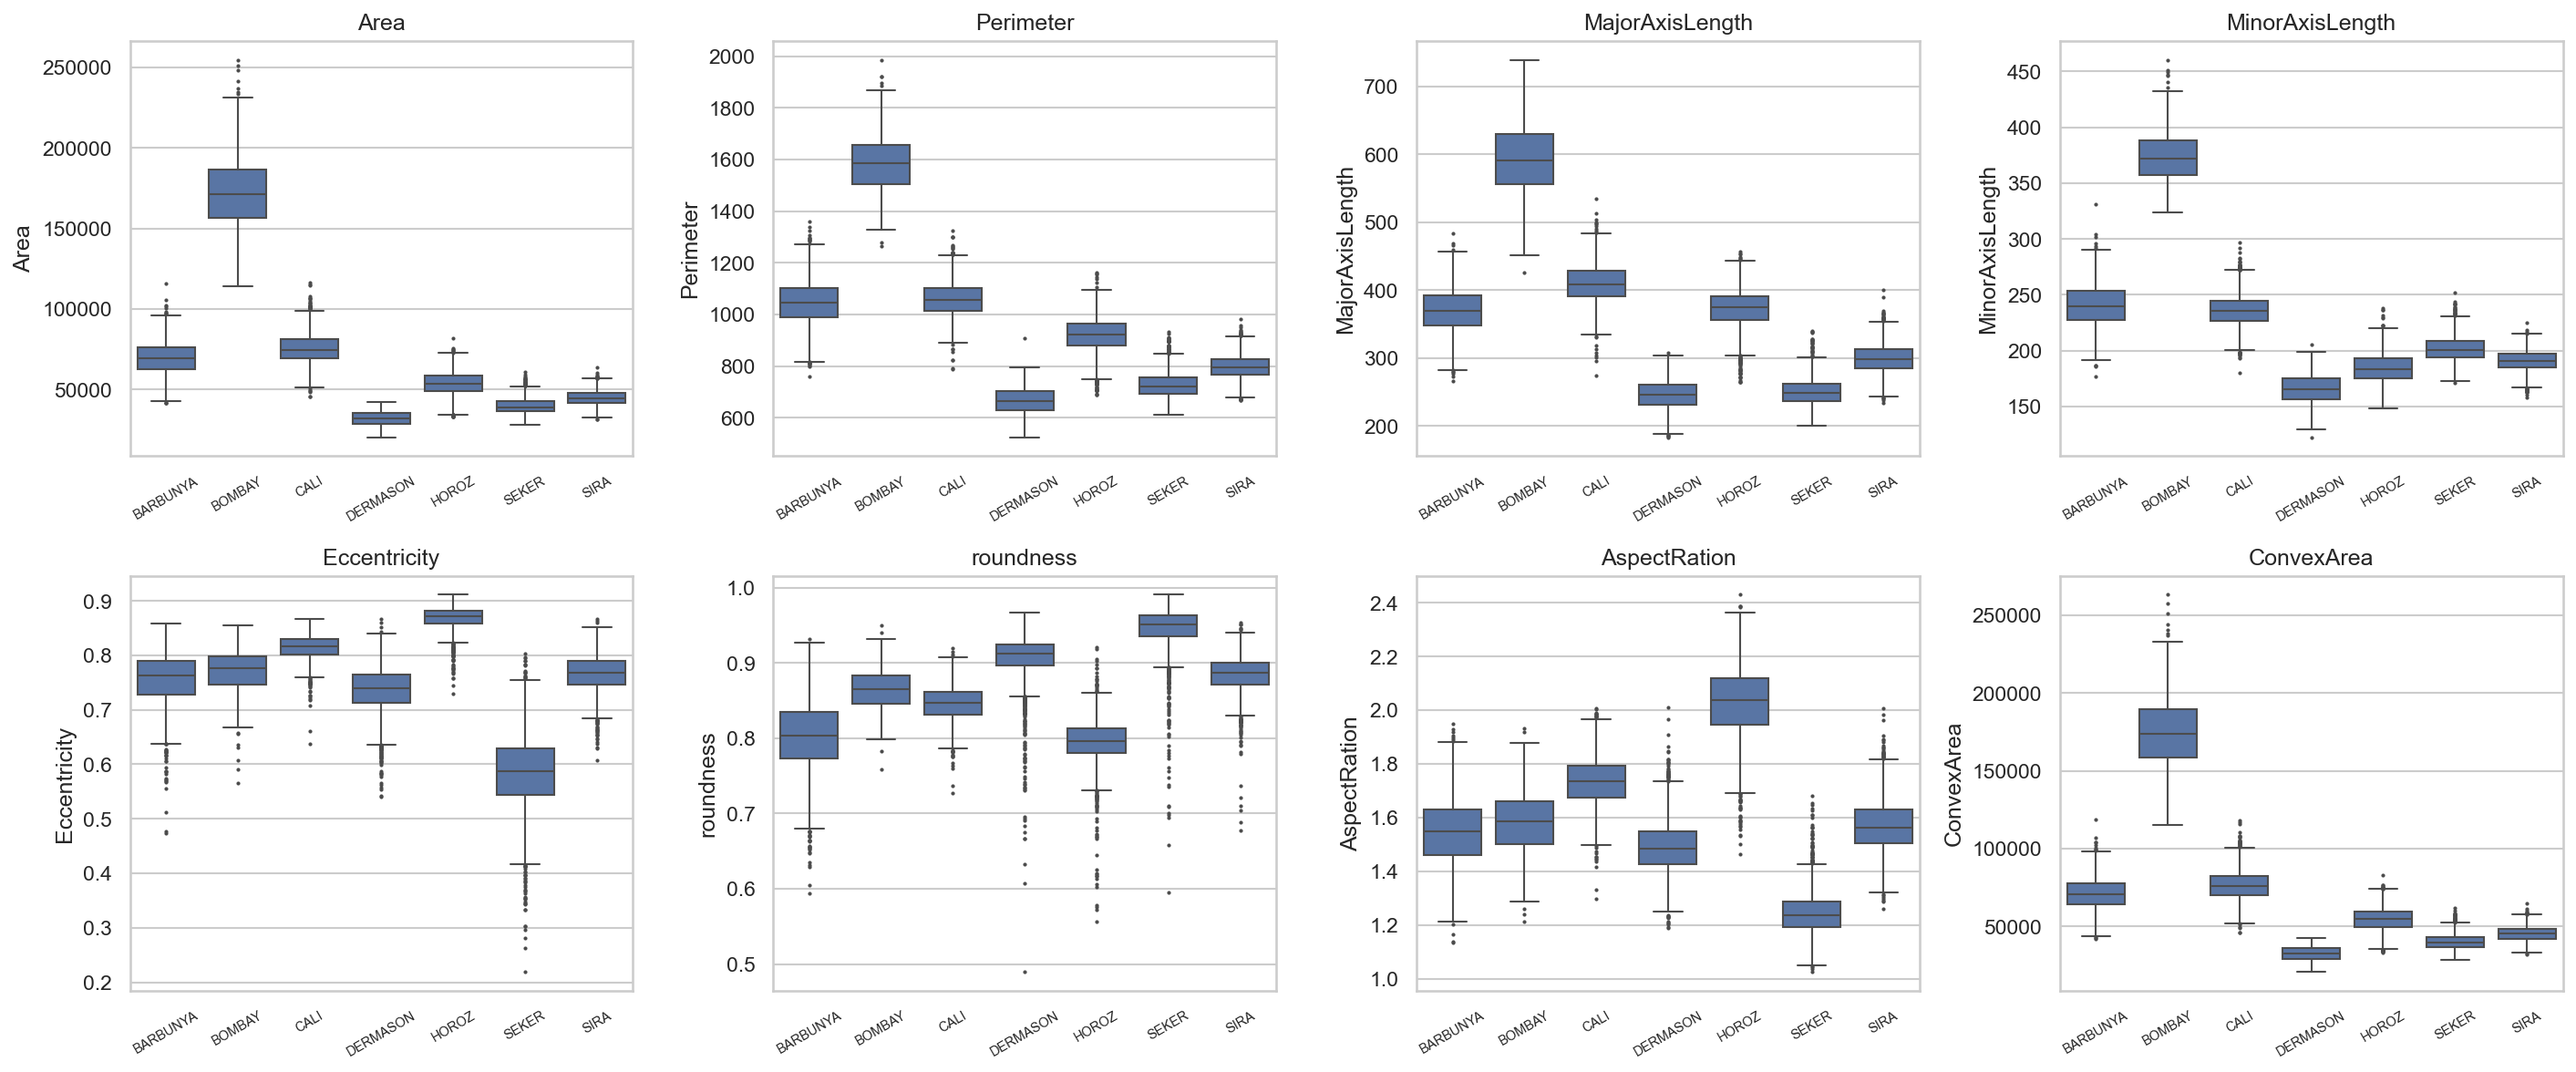
\includegraphics[width=\linewidth]{figures/q2_eda.png}
\caption{Feature distributions per variety. Bombay is far larger than the rest; Sira, Dermason and Seker overlap.}
\end{figure}

\textbf{b. Implementation.}
\begin{itemize}\itemsep0pt
\item \emph{Activations} --- sigmoid, tanh, ReLU and leaky ReLU, each with its derivative, written by hand. The output layer is softmax.
\item \emph{Forward pass} --- stores every pre-activation $z^l$ and activation $a^l$.
\item \emph{Backward pass} --- for softmax with cross-entropy the output error is $\hat y - y$; the error then propagates back as
$\delta^l = (\delta^{l+1}W^{l+1\top})\odot f'(z^l)$, with $\partial L/\partial W^l = a^{l\top}\delta^{l+1}$.
\item \emph{SGD} --- weights are updated after each shuffled mini-batch of 32 (lr 0.05, 60 epochs); \texttt{batch\_size=1} gives pure per-sample SGD.
\item \emph{Check} --- analytic gradients match central finite differences with relative error $2\times10^{-10}$.
\end{itemize}
The baseline 8--32--32--7 ReLU network reaches \textbf{91.3\% test accuracy}. Per variety: Bombay 100\%, Cali 94.7\%, Horoz 93.2\%,
Seker 91.1\%, Barbunya 90.9\%, Dermason 90.8\%, Sira 87.1\%.

\begin{figure}[H]\centering
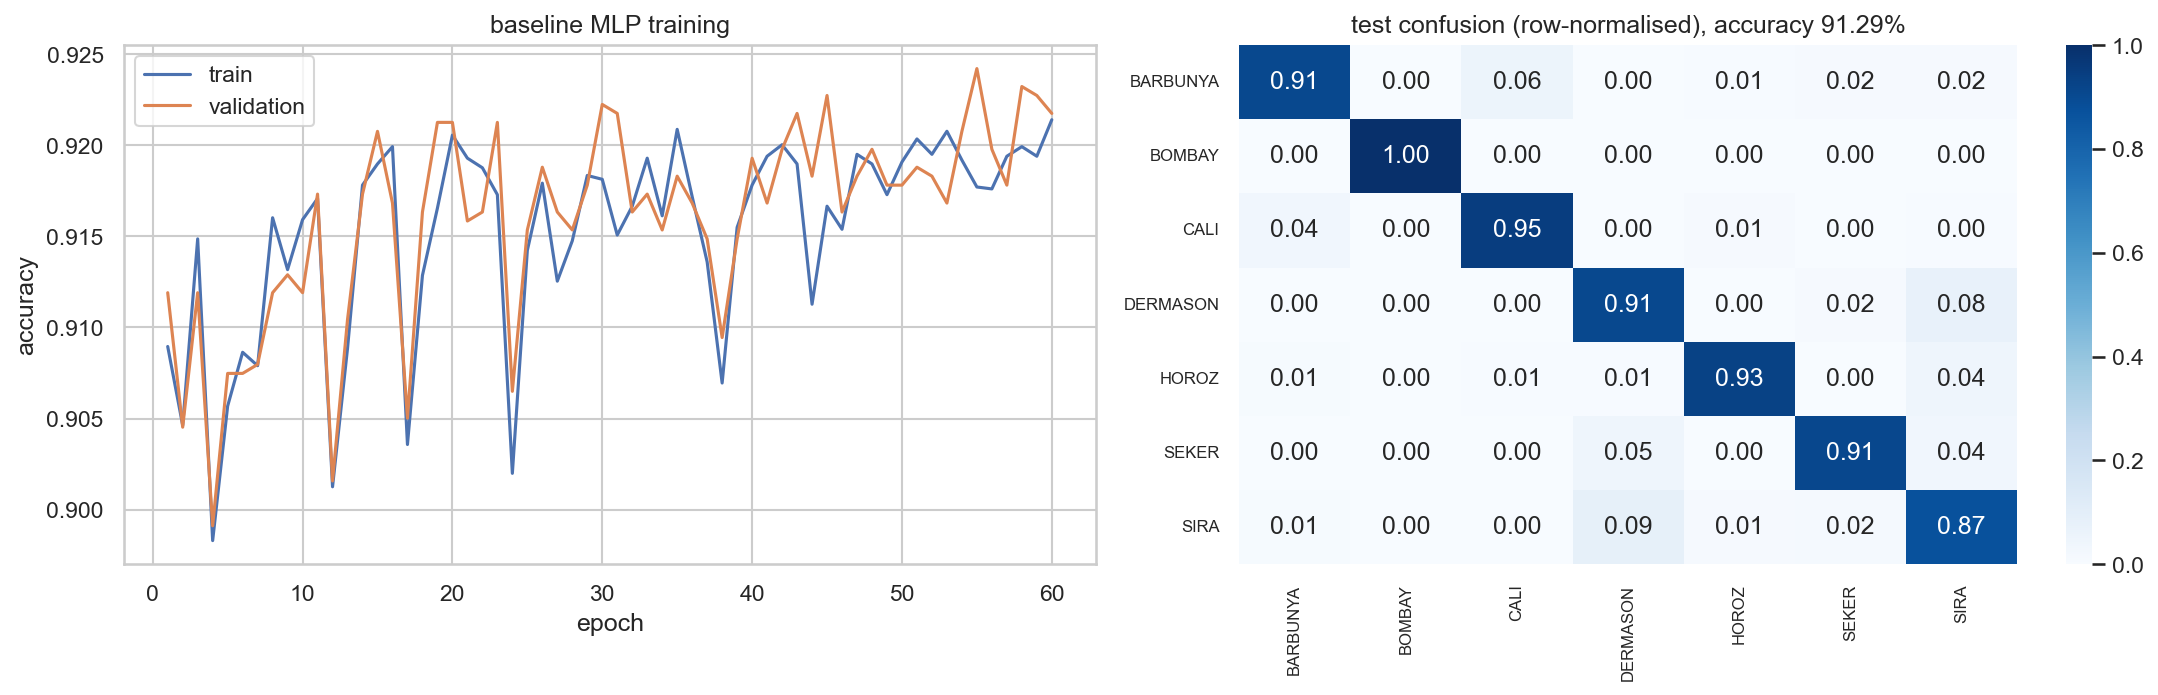
\includegraphics[width=\linewidth]{figures/q2_baseline.png}
\caption{Baseline training curve and test confusion matrix.}
\end{figure}
Most of the remaining errors are between Sira, Dermason and Seker, three similarly sized round beans whose shapes overlap in every feature.

\textbf{c. Activation functions} (same 8--32--32--7 network, 60 epochs):
\begin{table}[H]\centering
\begin{tabular}{lcccc}\toprule
Activation & Train acc. & Val acc. & Test acc. & Epochs to 90\% val.\\\midrule
sigmoid & 0.913 & 0.913 & 0.913 & 14\\
tanh & 0.921 & 0.920 & \textbf{0.914} & 1\\
ReLU & 0.921 & \textbf{0.922} & 0.913 & 1\\
leaky ReLU & 0.921 & 0.921 & 0.912 & 1\\\bottomrule
\end{tabular}
\end{table}
\begin{figure}[H]\centering
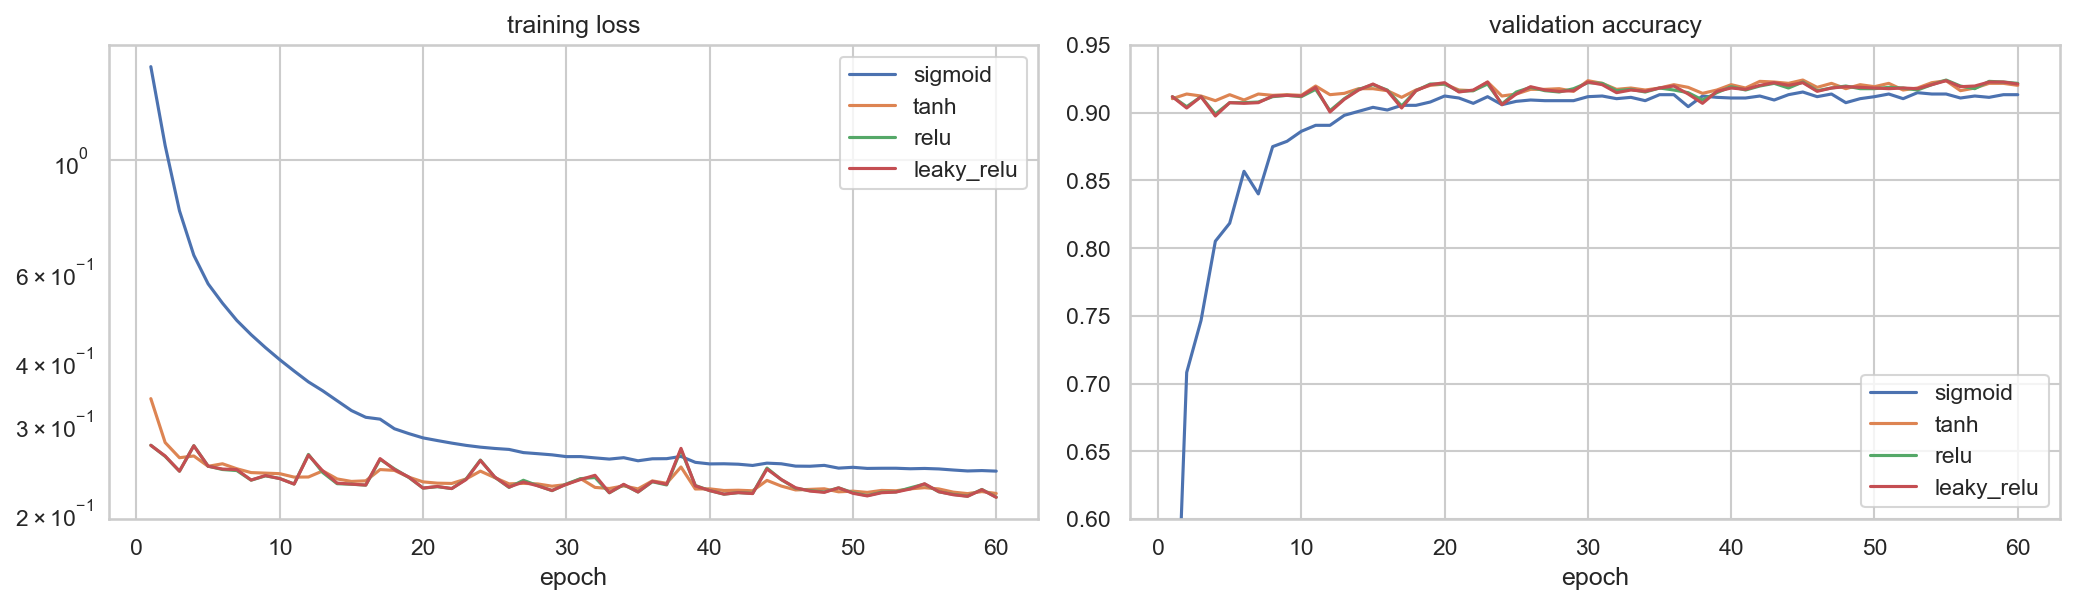
\includegraphics[width=\linewidth]{figures/q2_activations.png}
\caption{Training loss (log scale) and validation accuracy per activation (the ReLU and leaky-ReLU curves overlap).}
\end{figure}
The final accuracies are almost identical ($\pm0.2\%$), because the problem is easy enough that any non-linearity is enough. What differs is
\textbf{training speed}: sigmoid needs 14 epochs to reach 90\% while the others get there in the first epoch. Sigmoid's derivative is at most 0.25,
so the gradient shrinks by at least 4$\times$ at every layer, and its outputs are all positive, which makes successive updates zig-zag. Tanh is zero-centred with a
maximum derivative of 1, and ReLU passes the gradient through unchanged wherever it is active. ReLU and leaky ReLU behave the same here, because with good
initialisation few units die in a 32-wide layer.

\textbf{d. Weight initialisation.}
\begin{table}[H]\centering
\begin{tabular}{llcc}\toprule
Initialisation & Activation & Test acc. & Distinct hidden-unit behaviours (layer 1, of 32)\\\midrule
random (He / Xavier) & ReLU & \textbf{0.913} & 32\\
random (He / Xavier) & tanh & \textbf{0.914} & 32\\
zero & ReLU / tanh & 0.262 & 1\\
constant (0.5) & ReLU & 0.485 & 1\\
constant (0.5) & tanh & 0.388 & 1\\\bottomrule
\end{tabular}
\end{table}
\begin{figure}[H]\centering
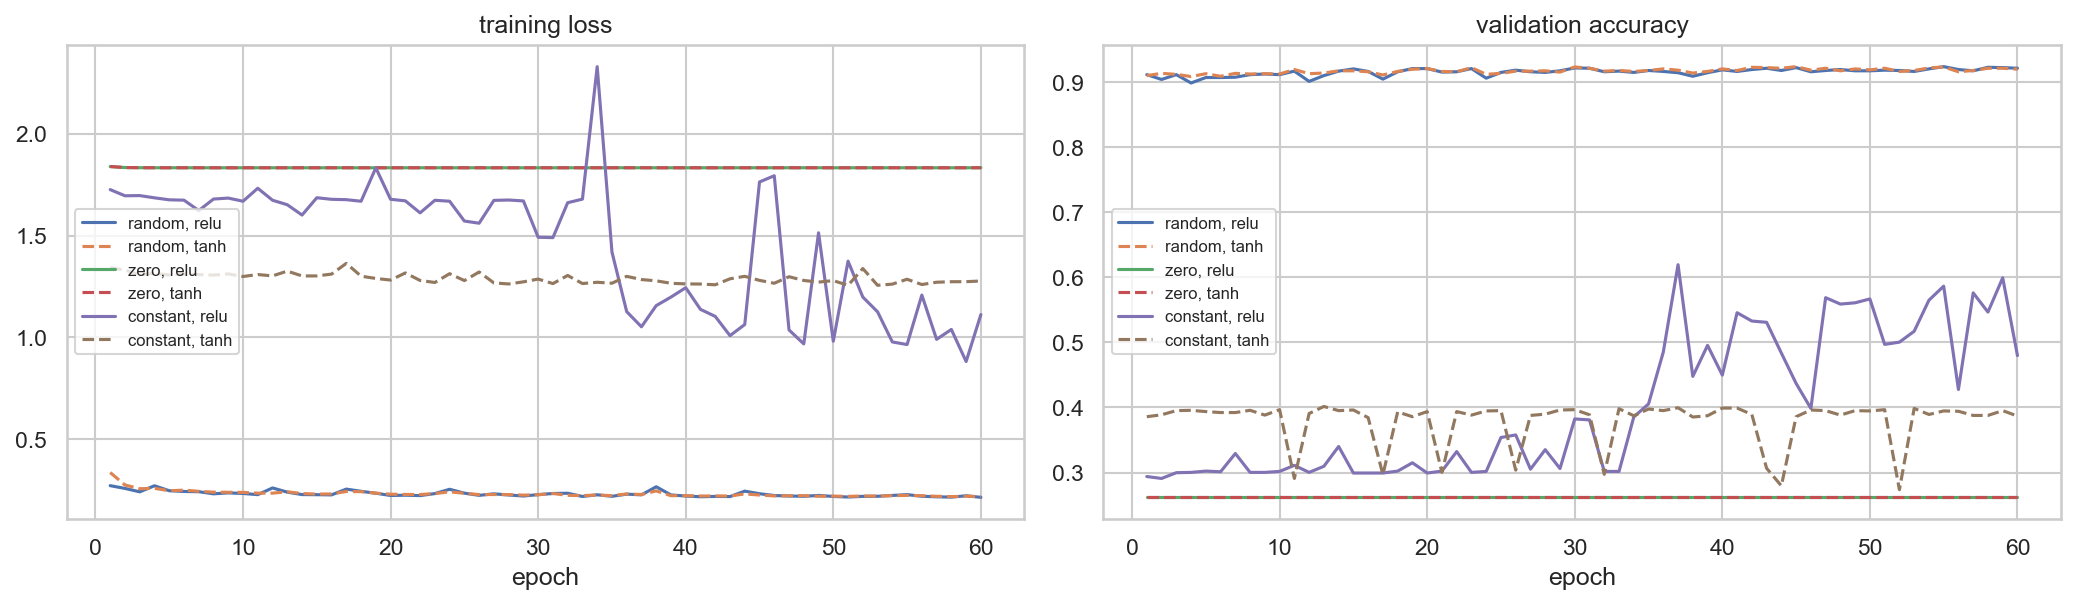
\includegraphics[width=\linewidth]{figures/q2_init.png}
\caption{Training loss and validation accuracy for each initialisation (solid: ReLU, dashed: tanh).}
\end{figure}
\textbf{Zero initialisation fails completely.} Every hidden unit outputs the same value; with ReLU and tanh that value is 0, so the
gradient reaching the hidden weights is exactly zero and they never move. Only the output bias learns, and the network always predicts the majority class
(Dermason, 26.2\%). \textbf{Constant initialisation} breaks the zero-gradient problem but not the \emph{symmetry}: all units in a layer start the same and
receive the same gradient, so they stay identical forever (1 distinct behaviour out of 32). The network behaves as if each hidden layer had a single neuron,
which explains the 39--49\% accuracy. Random initialisation gives each unit a different starting point; scaling it to the layer size (He for ReLU,
Xavier for tanh) keeps the activations and gradients at a sensible size.

\textbf{e. Number of hidden nodes} (two hidden layers of width $h$, ReLU):
\begin{table}[H]\centering
\begin{tabular}{rrcccr}\toprule
$h$ & Parameters & Train acc. & Val acc. & Test acc. & Time (s)\\\midrule
2 & 45 & 0.262 & 0.262 & 0.262 & 0.5\\
4 & 91 & 0.916 & 0.918 & 0.908 & 0.5\\
8 & 207 & 0.919 & 0.922 & 0.911 & 0.7\\
16 & 535 & 0.920 & 0.921 & 0.912 & 0.9\\
32 & 1575 & 0.921 & 0.922 & \textbf{0.913} & 1.1\\
64 & 5191 & 0.921 & 0.921 & 0.912 & 1.3\\
128 & 18567 & 0.922 & 0.922 & \textbf{0.913} & 1.9\\\bottomrule
\end{tabular}
\end{table}
\begin{figure}[H]\centering
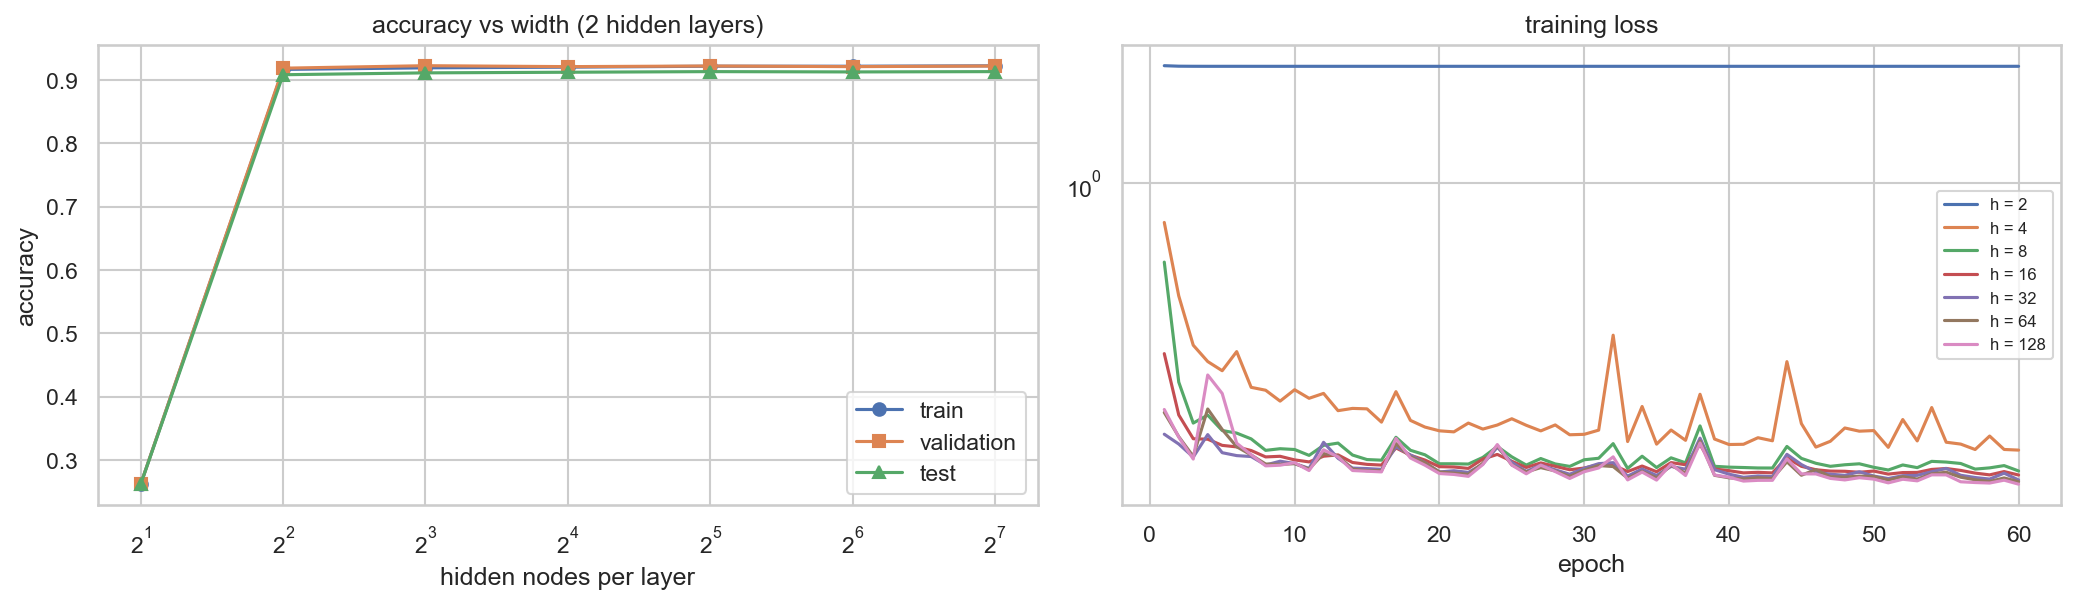
\includegraphics[width=\linewidth]{figures/q2_hidden.png}
\caption{Accuracy vs.\ width, and training loss per width.}
\end{figure}
Accuracy saturates very early: 4 hidden nodes already give 90.8\%, and going from 32 to 128 nodes (12$\times$ the parameters) changes nothing. The 8 inputs
are mostly redundant size measurements (correlations up to 0.99), so the useful decision function is low-dimensional. Wider networks
only make training slower, and train and validation accuracy stay equal, so with 9.5k samples there is no overfitting even at 18.5k parameters.
\textbf{$h=2$ is a failure case, not a capacity limit.} With only two ReLU units in the second layer, both died early in training (they output 0 for every
input), so no signal reached the output layer and it fell back to the majority class. Repeating this over 4 seeds, a width-2 ReLU network always lost at least one unit
(26--75\% accuracy), while the same tanh network, which cannot die, reached 71--87\%. Narrow ReLU layers are fragile because a single dead unit removes a
large share of the layer's capacity.

\textbf{f. Saving and loading.} \texttt{MLP.save} writes the layer sizes, the activation name and every weight matrix and bias vector to a single
\texttt{.npz} file, and \texttt{MLP.load} rebuilds the network from it. The restored model gives identical predictions on all 2032 test samples
(\texttt{mlp\_weights.npz} is saved alongside this report).

\end{document}
